
In this work, we quantified the effect of the super-sample covariance on the covariance matrix of higher-order statistics for a weak lensing survey. To achieve this, we conducted a series of N-body simulations and analyzed the resulting convergence maps. These maps enable the computation of covariance matrices for various statistical measures. Thus, we could investigate the impact of the super-sample covariance on these matrices.

In the following sections, we discuss the methodology used to generate the convergence maps, extract patches for analysis, incorporate noise, apply Gaussian smoothing, and compute the statistical measures. We also outline the process for estimating the covariance matrices and comparing the results between the BIGBOX and TILED simulations.

\section{Constructing the BIGBOX and TILED Datasets}
We employed the publicly available particle-mesh simulation code, \texttt{FASTPM} \citep{10.1093/mnras/stw2123}, to generate the simulations used in this study. As discussed in Section~\ref{sec:fastpm}, \texttt{FASTPM} was chosen to achieve high accuracy while minimizing computational time.

The two simulations used in this work are \textbf{BIGBOX} and \textbf{TILED}. For both simulations, we adopted the same cosmological parameters as those used in the IllustrisTNG project \citep{2019ComAC...6....2N}. The parameters are listed in Table~\ref{tab:simulations}.

\begin{table}[h]
    \centering
    \begin{tabular}{lcc}
    \toprule
    \textbf{Parameter} & \textbf{Symbol} & \textbf{Value} \\
    \midrule
    Hubble constant & $H_0$ & 67.74 \, [$\mathrm{km\,s^{-1}\,Mpc^{-1}}$] \\ 
    Matter density & $\Omega_m$ & 0.3089 \\
    Baryon density & $\Omega_b$ & 0.0486 \\
    Amplitude of fluctuations & $\sigma_8$ & 0.8159 \\
    Spectral index & $n_s$ & 0.9667 \\
    Sum of neutrino masses & $M_{\nu}$ & 0.0 \, [eV] \\
    \bottomrule
    \end{tabular}
    \caption{Cosmological parameters used in the N-body simulations.}\label{tab:simulations}
\end{table}

The BIGBOX simulation, conducted as part of the HalfDome project \citep{2024arXiv240717462B}, uses $6144^3$ particles within a box of side length $3750$ Mpc/h, employing periodic boundary conditions. The simulation volume is replicated approximately $2.6$ times per dimension to cover the redshift range $z = 0$ to $z = 4$, resulting in a total volume of about $10$ Gpc/h$^3$. At the maximum redshift considered in this work, $z = 2.5$, the simulation volume is replicated approximately $1.2$ times per dimension.

The TILED simulation covers a smaller volume with a side length of $L = 625$ Mpc/h, populated with $1024^3$ particles and also employing periodic boundary conditions. This combination of box size and particle number was chosen to match the resolution of the BIGBOX simulation. To cover the same redshift range as the BIGBOX simulation, the TILED box was replicated $10$ times along each axis, although $6$ replications are sufficient for the range $z = 0$ to $z = 2.5$. Figure~\ref{fig:simulationsetting} illustrates the spatial and redshift setup for the BIGBOX and TILED simulations employed in this cosmological study.

\begin{figure}[ht]
    \centering
    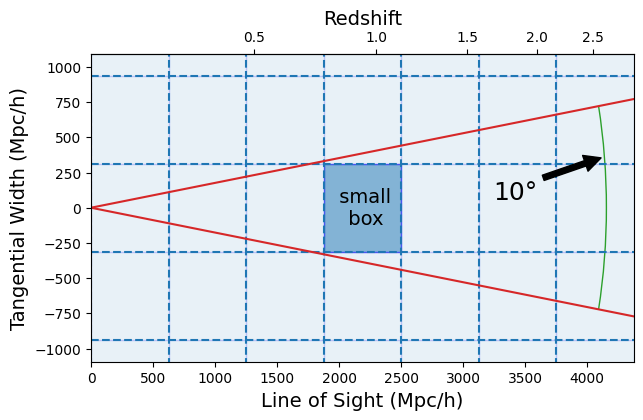
\includegraphics[width=0.8\textwidth]{figures/light_cone_configuration.png}
    \caption[Spatial and redshift setup for the BIGBOX and TILED simulations]{Spatial and redshift setup for the BIGBOX and TILED simulations. Dashed blue grids partition the overall simulation volume into smaller, manageable tiling regions, with each tile representing a replication of the TILED simulation. The lower horizontal axis indicates the line-of-sight distance in $\mathrm{Mpc}/h$, while the corresponding redshift values are displayed on the top axis.} \label{fig:simulationsetting}
\end{figure}

Both simulations commenced at an initial redshift of $z = 9$, utilizing an initial linear matter power spectrum at $z = 0$ generated via the \texttt{CLASS} code \citep{2011JCAP...07..034B}. The simulations were evolved over $60$ time steps to reach the present day ($z = 0$). The resulting particle distributions were output in $80$ shells spanning scale factors from $a = 0.2$ to $a = 1.0$, with a uniform spacing of $\Delta a = 0.01$. At each scale factor $a_i$, particles within the shells were projected onto a HEALPix grid \citep{Górski_2005} with $N_{\text{side}} = 8192$, providing an angular resolution of approximately $0.43$ arcminutes, to generate mass maps.

The BIGBOX and TILED simulations were executed on the TACC (Texas Advanced Computing Center) cluster. The BIGBOX simulations required approximately $4$ hours per realization, utilizing $2048$ nodes, while the TILED simulations were completed in $2$ hours per realization using $64$ nodes.

In total, we generated $11$ realizations of the BIGBOX simulation and $20$ realizations of the TILED simulation, each initialized with distinct random seeds. This ensemble of realizations enables us to robustly sample cosmic variance and ensures that our statistical analyses are not biased by the initial conditions of any single simulation.

It is important to note that the observer is positioned at the corner point shared by $8$ replicated boxes in both the TILED and BIGBOX simulations. This placement induces the Box Replication Effect, characterized by a kaleidoscope-like pattern of heavily tiled regions along the line of sight, particularly near the equatorial regions and in directions parallel to the box edges (see Figure~\ref{fig:boxreplication_patch} for $z = 1.5$). These replicated regions can introduce artificial correlations and anisotropies in the mass maps, potentially biasing our statistical measurements. To mitigate this effect, we exclude the most heavily tiled regions from our analysis, ensuring that the Box Replication Effect does not significantly impact our results. A detailed discussion of this phenomenon and its implications is provided in Section~\ref{sec:boxreplication}.

\begin{figure}[ht]
    \centering
    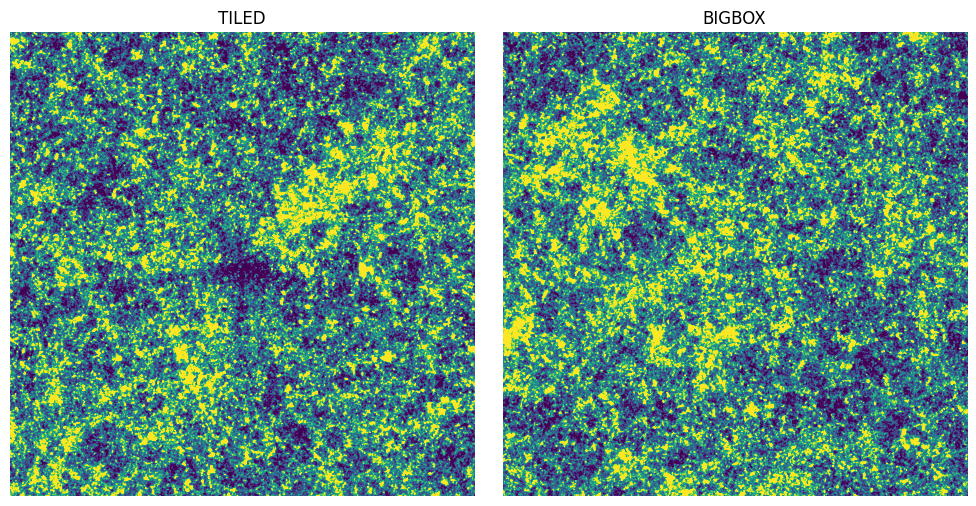
\includegraphics[width=\textwidth]{figures/samplepatch.png}
    \caption[Illustration of a $5 \times 5$ patch at $z = 1.5$]{Illustration of a $5 \times 5$ patch around $(\theta, \phi) = (\pi/2, 0)$ extracted from the TILED and BIGBOX simulations at $z = 1.5$. The TILED simulation displays a distinct kaleidoscope-like pattern caused by box replication, resulting in heavily tiled regions along the line of sight and near the equator. This pattern becomes more pronounced at higher redshifts.}
    \label{fig:boxreplication_patch}
\end{figure}

\section{Producing Weak Lensing Convergence Maps at Multiple Redshifts}
Since we already have the projected mass map at each scale factor, we calculate the convergence map at each redshift following the discussion in Sections~\ref{sec:convergence} and~\ref{sec:weak-lensing-generation}. As the difference between the TILED and BIGBOX simulations due to the super-sample effect becomes apparent around redshift $z \approx 1$, it is worthwhile to examine the contribution from each redshift to the convergence map.

Figure~\ref{fig:lensing_efficiency} shows the normalized lensing efficiency as a function of comoving distance (in Mpc/$h$) for multiple source redshifts ($z$). The lensing efficiency curves exhibit distinct peaks at intermediate comoving distances, highlighting the regions where the matter distribution along the line of sight most significantly enhances the gravitational lensing signal

\begin{figure}[ht]
    \centering
    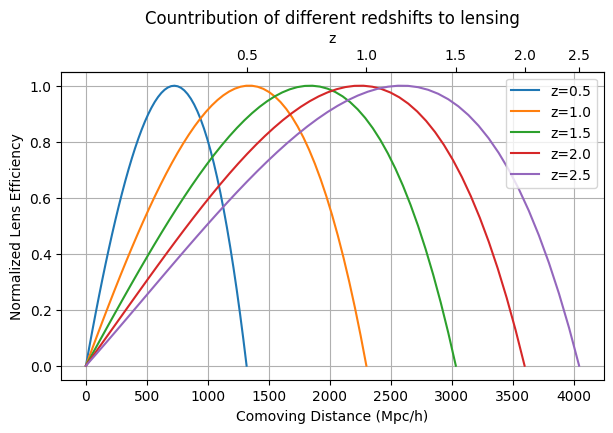
\includegraphics[width=0.8\textwidth]{figures/lensefficiency.png}
    \caption[Normalized lensing efficiency for multiple source redshifts]{Normalized lensing efficiency as a function of comoving distance for multiple source redshifts. The efficiency curves peak at intermediate comoving distances, indicating regions where the matter distribution enhances the gravitational lensing signal.}
    \label{fig:lensing_efficiency}
\end{figure}

We considered source redshifts $z_s = [0.5, 1.0, 1.5, 2.0, 2.5]$, covering the range of distances relevant for both current and upcoming galaxy surveys. At low redshifts ($z < 1$), both the BIGBOX and TILED simulations are affected by super-sample effects. However, at higher redshifts ($z > 1$), these effects become more pronounced in the BIGBOX simulation. This divergence occurs because, at approximately $z = 1$, the light cone in the TILED simulation begins to extend tangentially across multiple replicated boxes. As a result, no additional super-survey modes arise within the TILED simulation beyond this redshift, effectively mitigating the influence of super-sample covariance.

Figure~\ref{fig:convergence_maps} shows the convergence maps generated from both the BIGBOX and TILED simulations for a source redshift of $z_s = 1.5$. These maps are depicted on \textsc{Healpix} grids with $N_{\text{side}} = 8192$, consistent with the methodology described.

\begin{figure}[ht]
    \centering
    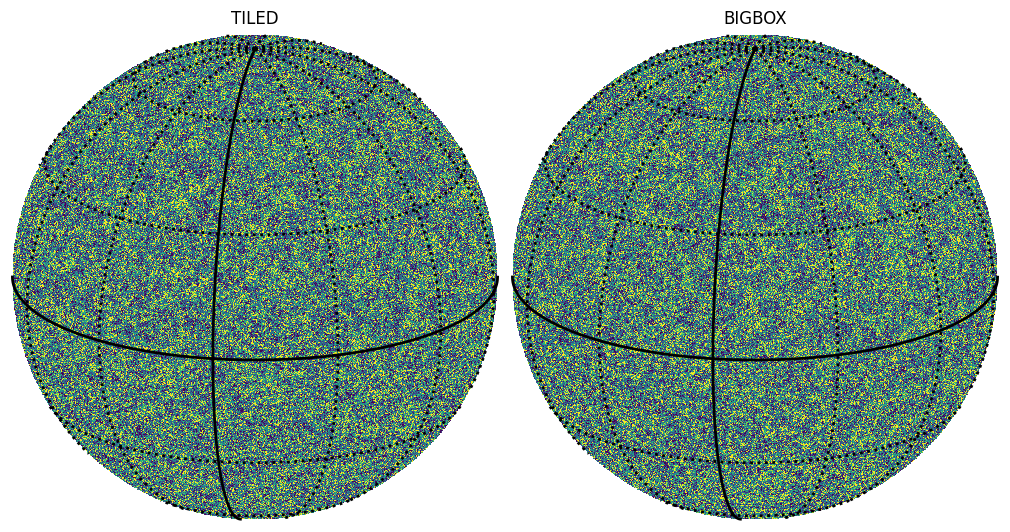
\includegraphics[width=\textwidth]{figures/samplemap.png}
    \caption[Convergence maps from the BIGBOX and TILED simulations]{Convergence maps from the BIGBOX and TILED simulations for source redshift $z_s = 1.5$. Yellow regions indicate positive convergence, while blue regions represent negative convergence. The maps exhibit similar large-scale structures, highlighting the agreement in the overall distribution of matter.}
    \label{fig:convergence_maps}
\end{figure}

\section{Incorporating Galaxy Shape Noise into Convergence Maps}
In actual observations, measurements of the lensing signal are affected by noise arising from the intrinsic shapes of galaxies and inaccuracies in shape measurements. This type of noise, known as shape noise, is a major source of uncertainty, especially on small angular scales. For example, shape noise can differ the number densities by approximately $12 \%$ in the HSC shear catalog (See Section 5.2 of \citealt{2018PASJ...70S..25M}). 

We considered four different surveys with varying galaxy number densities, as detailed in Table~\ref{tab:survey_comparison}. The variance of the shape noise per pixel was calculated using the following expression:
\begin{equation}
    \sigma_{\kappa, \text{noise}}^2 = \frac{\sigma_{\epsilon}^2}{2 n_{\mathrm{gal}} A_{\mathrm{pix}}},
\end{equation}
where $\sigma_{\epsilon}$ is the intrinsic ellipticity dispersion of galaxies, set to $\sigma_{\epsilon} = 0.26$ \citep{2019A&A...627A..59E}, $n_{\mathrm{gal}}$ is the galaxy number density per square arcminute, and $A_{\mathrm{pix}}$ is the solid angle of a pixel, set to $0.43$ arcminutes$^2$. Using this calculated variance, we generated a Gaussian random field, $n(\hat{\mathbf{n}})$, and added it to the convergence maps to simulate the observed signal:
\begin{equation}
    \kappa_{\mathrm{obs}}(\hat{\mathbf{n}}) = \kappa(\hat{\mathbf{n}}) + n(\hat{\mathbf{n}}).
\end{equation}

\section{Patch Selection and Projection} \label{sec:patch_selection}
To simplify the analysis onto a flat patch, we extracted $10^\circ \times 10^\circ$ patches from the full-sky convergence maps. To maximize the number of uniformly distributed patches without repetition, we employed a Fibonacci grid \citep{2006QJRMS.132.1769S, 2023MNRAS.524.5591F} for extracting patches from the full-sky map. The center of each patch was positioned at the vertices of the Fibonacci grid, defined by golden ratio spirals:
\begin{equation}
    \sin \theta_i = \frac{2i}{2N + 1}, \quad \phi_i = \frac{2 \pi i}{\varphi}, \quad -N \leq i \leq N, \quad -\frac{\pi}{2} \leq \theta_i \leq \frac{\pi}{2},
\end{equation}
where $N$ is the number of patches and $\varphi = (1 + \sqrt{5})/2$ is the golden ratio. The visualization of the Fibonacci grid is shown in Figure~\ref{fig:fibonacci}.
\begin{figure}[ht]
    \centering
    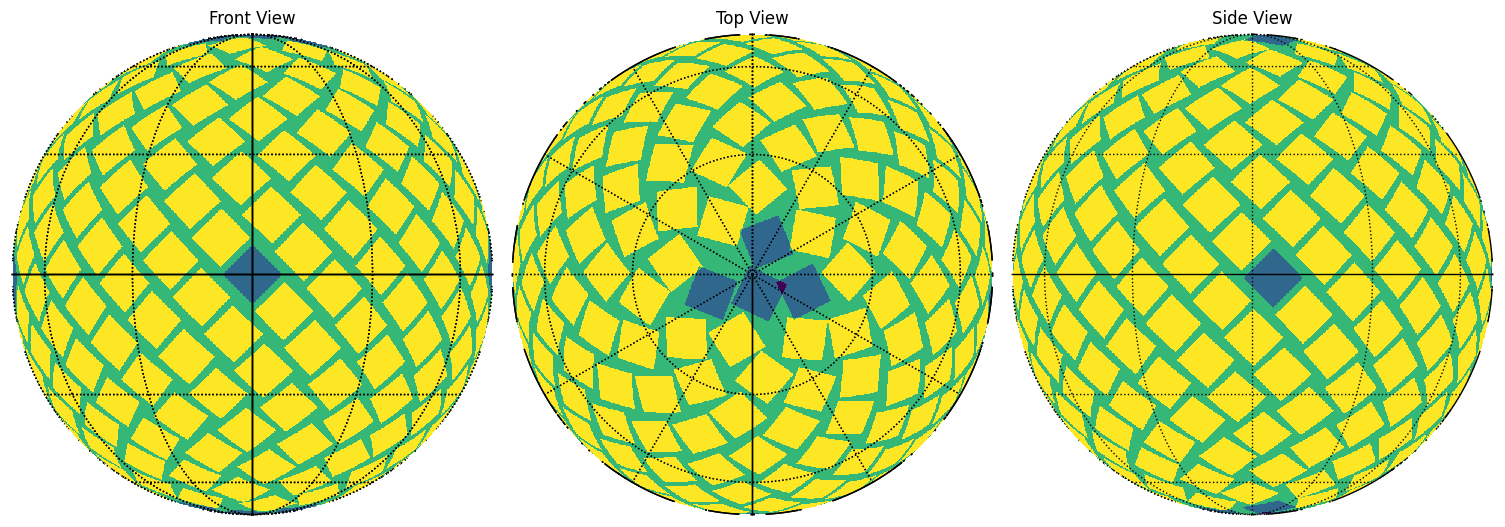
\includegraphics[width=\textwidth]{figures/fibonacci_grid.png}
    \caption[Visualization of the Fibonacci grid]{Visualization of the Fibonacci grid with $N_{\text{patches}} = 273$, where each patch covers approximately $10^\circ \times 10^\circ$. After optimization and masking, the number of patches is reduced to $N_{\text{patches}} = 194$, effectively covering $47\%$ of the sky. Each panel shows the patch distribution from a front view, top view, and the final front view after masking.}
    \label{fig:fibonacci}
\end{figure}
Following \citet{2023MNRAS.524.5591F}, the maximum number of patches can be obtained by aligning the diagonals of square patches with the longitude lines. However, due to programming constraints, we extracted patches with their sides aligned to the latitude lines. To achieve the desired $10^\circ \times 10^\circ$ shape, we first extracted patches with a larger side length and then rotated and cropped them accordingly.

Before extracting the patches, we optimized the number of patches to be extracted from the full-sky map. The number of patches, denoted \( N_{\text{patches}} \), was determined to ensure that individual patches do not overlap, except in regions near the poles, where overlapping patches were subsequently discarded. Each patch on the full-sky map is defined as:
\begin{align}
    \left( \theta_i - R_{\text{patch}},\, \phi_i + R_{\text{patch}} \sin \theta_i \right),  \quad & \left( \theta_i + R_{\text{patch}},\, \phi_i + R_{\text{patch}} \sin \theta_i \right), \nonumber \\
    \left( \theta_i - R_{\text{patch}},\, \phi_i - R_{\text{patch}} \sin \theta_i \right), \quad &
    \left( \theta_i + R_{\text{patch}},\, \phi_i - R_{\text{patch}} \sin \theta_i \right)
\end{align}
with \( R_{\text{patch}} = 5\sqrt{2}\, \mathrm{\deg} \), the half diagonal length of the patch.
The optimization process began with an initial count of \( N_{\text{patches}} = 400 \) and involved iteratively reducing this number until a configuration was achieved in which patches remained non-overlapping, except for centers located within \( 2R_{\text{patch}}\) of the poles. Specifically, the thresholds $|\theta_i| \geq 2R_{\text{patch}}$ and $|\phi_i| \leq \pi - 2R_{\text{patch}}$ were applied to ensure that the patches did not include the poles.

After optimization and masking, the number of patches was reduced to $N_{\text{patches}} = 273$, further decreasing to $N_{\text{patches}} = 265$ to effectively cover $64 \%$ of the sky. Additionally, patches containing points heavily tiled along the line of sight were excluded to mitigate the severe Box Replication Effect (see Section~\ref{sec:boxreplication} for further details). Consequently, the final number of patches used for analysis was $N_{\text{patches}} = 194$, effectively covering $47 \%$ of the sky.

For a Fibonacci grid center characterized by coordinates \( (\theta_i, \phi_i) \), we first employed the \texttt{gnomview} function from the \texttt{healpy} library \citep{Zonca2019} to project each spherical patch onto a flat plane using a gnomonic projection. Each patch was then rotated by $45^\circ$ around its center to align the diagonal of the patch with the longitude lines. Finally, the patch was cropped according to the corresponding vertices to achieve the desired shape. Figure~\ref{fig:fibonacci_extraction} illustrates the process of extracting a patch from the full-sky convergence map and the additional steps taken to obtain the final patch.
\begin{figure}[ht]
    \centering
    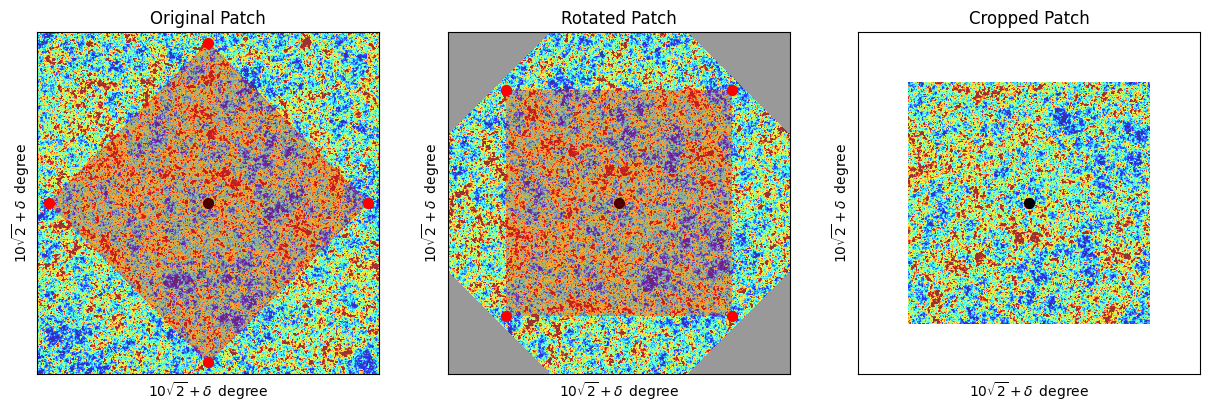
\includegraphics[width=\textwidth]{figures/fibonacci_extraction.png}
    \caption[Extraction of a patch from the full-sky convergence map using a Fibonacci grid]{Extraction of a patch from the full-sky convergence map using a Fibonacci grid. The patch covers an area of $10^\circ \times 10^\circ$ and is centered at a vertex of the Fibonacci grid. From left to right, the panels show the originally extracted patch, the patch rotated $45^\circ$ around its center, and the final patch after a second rotation. The red-shaded region represents the final patch used for analysis.}
    \label{fig:fibonacci_extraction}
\end{figure}

Each patch is represented by a $2048 \times 2048$ grid of pixels, resulting in a pixel size of:
\begin{equation}
    \Delta \theta = \frac{10^\circ}{2048} \approx 0.00488^\circ \approx 0.293' \quad \text{per pixel}.
\end{equation}
For each realization, the covariance was computed using 194 patches extracted from the full-sky map of each simulation. This resulted in a total of 2134 patches from the BIGBOX simulation and 3880 patches from the TILED simulation. This ensemble of patches enables us to robustly sample both cosmic variance and shot noise, ensuring that our statistical analyses are sufficient for the power spectrum at $\ell = 5283$ and peak counts in $ \kappa \in \left[-0.06, 0.45\right]$ \citep{2016PhRvD..93f3524P}.

\section{Applying Gaussian Kernels to Convergence Fields}
Shape noise predominantly affects small angular scales. To mitigate this noise and enhance the detection of the underlying lensing signal, we applied Gaussian smoothing to the noisy convergence maps. The Gaussian filter is defined as:
\begin{equation}
    W(\theta) = \frac{1}{\pi \theta_{\mathrm{G}}^2} \exp\left( -\frac{\theta^2}{\theta_{\mathrm{G}}^2} \right),
\end{equation}
where $\theta$ is the angular distance from the center of the filter, and $\theta_{\mathrm{G}}$ is the smoothing scale. For our analysis, we selected $\theta_{\mathrm{G}} = 2'$, $5'$, $8'$, and $10'$.

By convolving the noisy convergence map with the Gaussian filter, we obtained the smoothed convergence map:
\begin{equation}
    \kappa_{\mathrm{smoothed}}(\hat{\mathbf{n}}) = \int d\Omega' \, W(|\hat{\mathbf{n}} - \hat{\mathbf{n}}'|) \kappa_{\mathrm{obs}}(\hat{\mathbf{n}}').
\end{equation}

Figure~\ref{fig:smoothing} illustrates the impact of Gaussian smoothing on a noisy convergence map, demonstrating the progressive suppression of small-scale fluctuations. The figure consists of four panels, each corresponding to a different smoothing scale: $\theta_{\mathrm{G}} = 2'$, $5'$, $8'$, and $10'$. As the smoothing scale increases, the Gaussian kernel increasingly attenuates small-scale noise, reducing the amplitude of fluctuations in the map. Although this process naturally diminishes the power spectrum at small angular scales, smoothing scales below $10'$ are sufficient to mitigate shape noise while retaining the non-Gaussian structures of the convergence field.
\begin{figure}[ht]
    \centering
    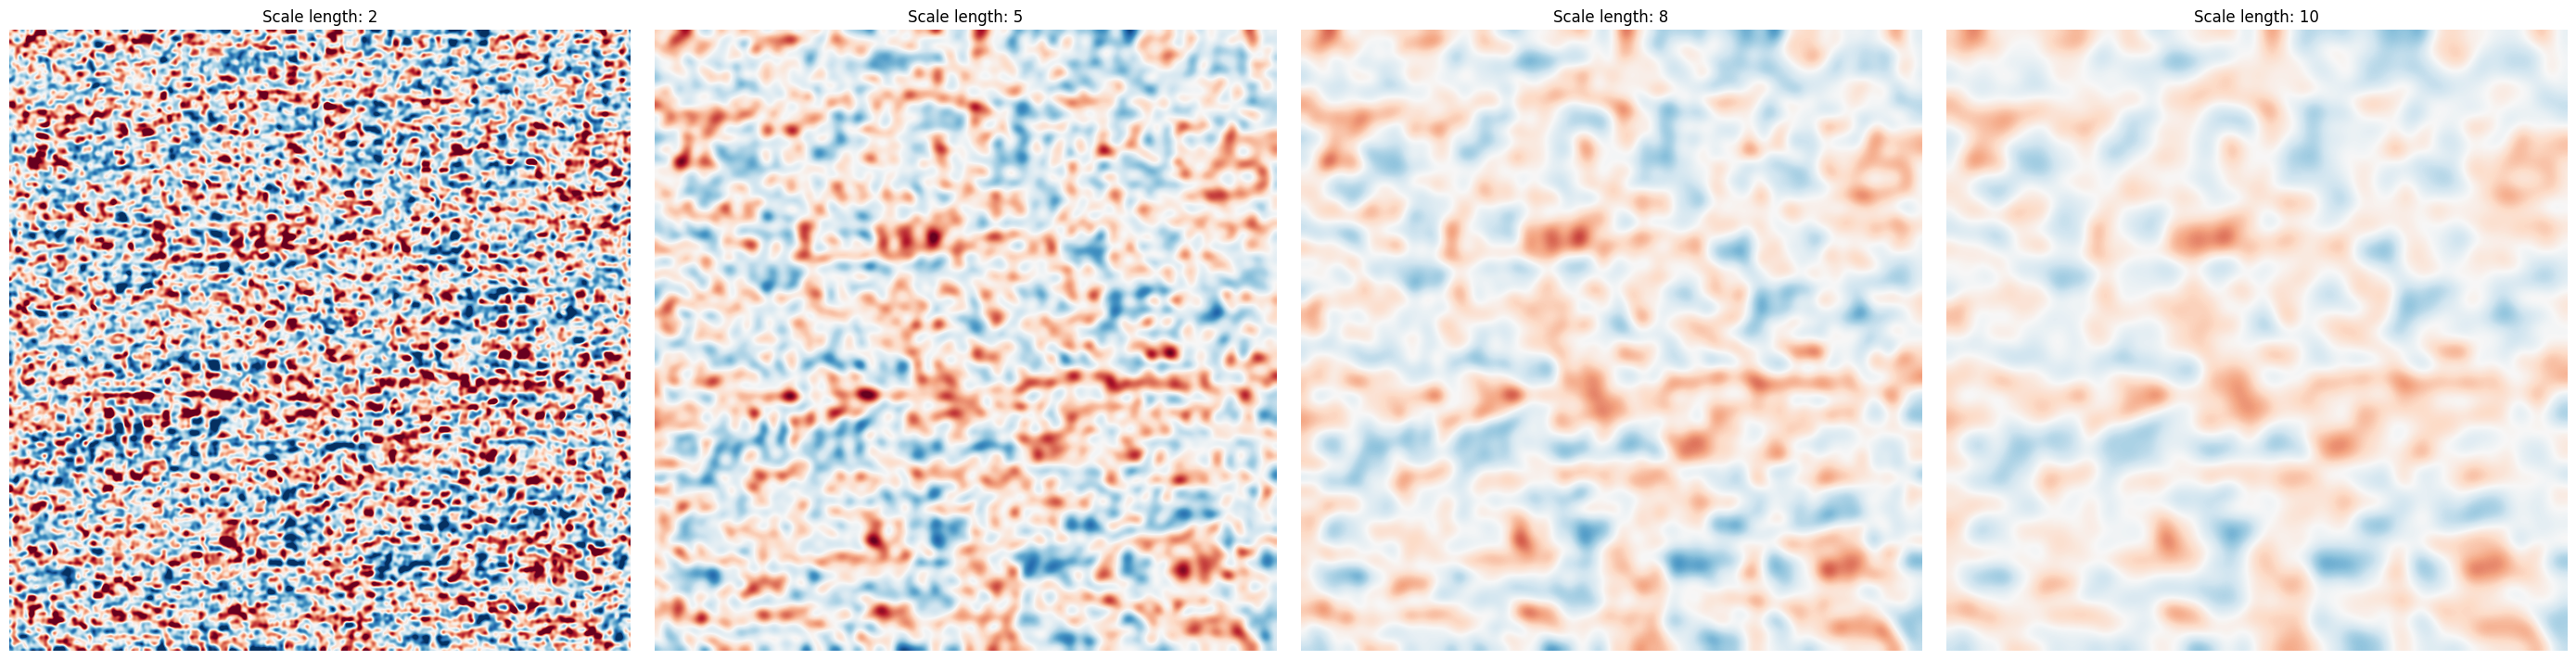
\includegraphics[width=\textwidth]{figures/smoothed_comparison.png}
    \caption[Gaussian smoothing on a noisy convergence map for multiple smoothing scales]{Effect of Gaussian smoothing on a noisy convergence map. Each panel shows the result of applying a Gaussian filter with a smoothing scale of \(\theta_{\mathrm{G}} = 2'\), \(5'\), \(8'\), or \(10'\). As the smoothing scale increases, small-scale noise is progressively suppressed, making large-scale structures more prominent. This demonstrates how Gaussian smoothing effectively reduces shape noise while preserving the underlying lensing signal.}
    \label{fig:smoothing}
\end{figure}

For the analysis of non-Gaussian statistics, we employ a Gaussian smoothing procedure, after which the statistics are computed from the resulting smoothed convergence maps. The application of a smoothing kernel effectively suppresses small-scale structures, thereby modifying the range of $\kappa$ values. To avoid the smoothing issues and the complex binning to consider, we normalize $\kappa$ values by the standard deviation of each patch's convergence map, $\sigma_{\kappa}$. 

Figure~\ref{fig:avg_sigma0} shows the mean standard deviation of the noiseless convergence maps obtained from both the BIGBOX and TILED simulations. While there is no significant difference between the two simulations, the standard deviation increases with both redshift and smoothing scale. The observed increase with redshift reflects the inclusion of additional shells along the line of sight, leading to greater variability in density contrasts. Similarly, the increase with smoothing scale arises from the smoothing process itself, which suppresses small-scale structures and amplifies the variability of larger-scale fluctuations.

\begin{figure}[ht]
    \centering
    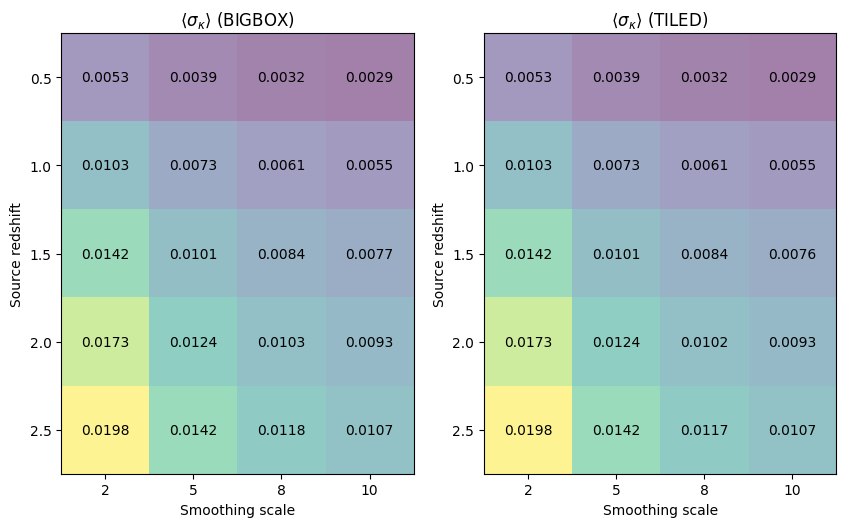
\includegraphics[width=\textwidth]{figures/avg_sigma0.png}
    \caption[Average standard deviation of noiseless convergence maps]{Average standard deviation of the noiseless convergence maps for the BIGBOX and TILED simulations. The standard deviation increases with both redshift and smoothing scale, with only subtle differences observed between the BIGBOX and TILED simulations.}
    \label{fig:avg_sigma0}
\end{figure}

\section{Extracting Weak Lensing Statistics from Convergence Maps}
To characterize the influence of super-sample covariance on higher-order statistics, this study focuses on the bispectrum, probability distribution function (PDF), peak counts, minima counts, and Minkowski functionals.

Table~\ref{tab:statistics} summarizes the range of values and the computational subroutines employed for each statistical measure.
\begin{table*}[htbp]
    \centering
    \begin{tabular}{lcc}
    \toprule
    \textbf{Statistic} & \textbf{Range} & \textbf{Subroutine (Sky Patch)} \\
    \midrule
    Angular Power Spectrum & $300 \leq \ell \leq 3000$ & \texttt{lenstools.powerSpectrum} \\
    Bispectrum & $300 \leq \ell \leq 3000$ & \texttt{lenstools.bispectrum} \\
    Peak Counts & $-4 \leq \kappa/\sigma_\kappa \leq 4$ & \texttt{lenstools.peakCount} \\
    Minima Counts & $-4 \leq \kappa/\sigma_\kappa \leq 4$ & \texttt{lenstools.peakCount} \\
    Probability Distribution Function (PDF) & $-4 \leq \kappa/\sigma_\kappa \leq 4$ & \texttt{lenstools.pdf} \\
    Minkowski Functionals & $-4 \leq \kappa/\sigma_\kappa \leq 4$ & Custom implementation \\
    \bottomrule
    \end{tabular}
    \caption{Summary of the statistical measures employed in this study, including their respective value ranges and the computational subroutines used for analysis.}
    \label{tab:statistics}
\end{table*}

\subsection{Angular Power Spectrum}
The angular power spectrum ($C_{\ell}^{\kappa\kappa}$) is estimated directly from the simulated convergence maps using \texttt{lenstools} \citep{2016A&C....17...73P}, without any preliminary smoothing. The considered multipole range spans from $\ell = 300$ to $\ell = 3000$, partitioned into eight logarithmically spaced bins. This binning scheme is chosen to maintain consistency with the multipole selection used in the Hyper Suprime-Cam Year 3 (HSC Y3) cosmic shear analysis \citep{2023PhRvD.108l3519D}. 

The lower limit of $\ell = 300$ excludes large-scale modes, as the primary focus of this study is on higher-order statistics, which are most sensitive to intermediate and small angular scales. Conversely, the upper limit of $\ell = 3000$ ensures the inclusion of small-scale modes where the super-sample effect becomes increasingly significant. Furthermore, this multipole range is robust given the sampling of simulated maps, as discussed in Section~\ref{sec:patch_selection}.

For benchmarking, we compute the theoretical angular power spectrum using the \texttt{Halofit} model \citep{2012ApJ...761..152T} and compare it with the measured angular power spectrum. The theoretical prediction is generated using the same set of cosmological parameters as those employed in the simulations.

\subsection{Bispectrum}
The bispectrum ($B_{\ell}$) is computed from the unsmoothed convergence maps using \texttt{lenstools}. We consider three distinct configurations: equilateral ($\ell_1 = \ell_2 = \ell_3$), squeezed ($\ell_1 = \ell_2 = 10\ell_3$), and isosceles ($\ell_1 = \ell_2 = 2\ell_3$). These configurations are chosen to capture different shapes of the bispectrum, providing complementary information about the underlying matter distribution.

The bispectrum computations are confined to the same multipole range as the angular power spectrum, specifically $\ell \in [300, 3000]$,  divided into eight logarithmically spaced bins. Although the bispectrum is more sensitive to noise and small-scale structures, maintaining an identical multipole range facilitates direct comparison with the angular power spectrum results.

For theoretical validation, we compute the bispectrum prediction using the \texttt{BiHalofit} model \citep{2020ApJ...895..113T} and compare it with the measured bispectrum from the simulations. The theoretical bispectrum is derived using the same cosmological parameters as those employed in the simulations.

\subsection{PDF}
We compute the probability distribution function (PDF) of the convergence field using \texttt{lenstools}. Each PDF is derived from the smoothed convergence maps over a normalized range of $-4 \leq \kappa/\sigma_{\kappa} \leq 4$, divided into eight equally spaced bins. Here, $\sigma_{\kappa}$ represents the standard deviation of the convergence field within each individual patch. This range is chosen to align with the study by \citet{2023arXiv230405928T}, while the binning is optimized to ensure that each bin contains a sufficient number of data points.

The theoretical prediction for the PDF is generated using the \texttt{hmpdf} code \citep{2020PhRvD.102l3545T}, employing the same linear matter power spectrum as that used in the simulations. The theoretically predicted PDF is then compared with the measured PDF to evaluate the consistency and accuracy of the underlying cosmological model and its assumptions.

\subsection{Peak/Minima Counts}
Peak and minima counts are computed from the smoothed convergence maps using \texttt{lenstools}, utilizing the same normalized range as the PDF: $-4 \leq \kappa/\sigma_{\kappa} \leq 4$, divided into eight evenly spaced bins. While the highest and lowest peaks are represented by relatively few data points, these extreme bins are retained to ensure consistency with the binning scheme adopted for the PDF.

\subsection{Minkowski Functionals}
The Minkowski functionals are calculated from the smoothed convergence maps using a custom implementation that adheres closely to the definitions outlined in Section~\ref{sec:minkowski_functionals}. As with the PDF and peak/minima counts, these functionals are computed over the normalized range $-4 \leq \kappa/\sigma_{\kappa} \leq 4$, divided into eight linearly spaced bins.

Figure~\ref{fig:avg_sigma1} illustrates the variance of the gradient field, $\sigma_1 = \sqrt{\kappa_x^2 + \kappa_y^2}$, which is a critical input for calculating the Minkowski functionals. As the smoothing scale increases, $\sigma_1$ decreases, reflecting the reduced influence of small-scale structures. Differences between the BIGBOX and TILED simulations, as well as across varying redshifts, remain subtle, highlighting the robustness of these measures and their relative insensitivity to large-scale environmental variations.

\begin{figure}[ht]
    \centering
    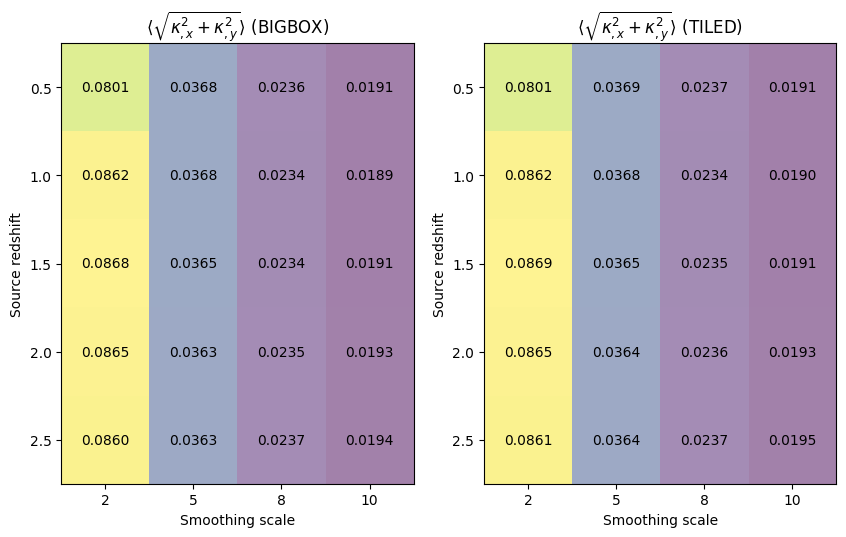
\includegraphics[width=\textwidth]{figures/avg_sigma1.png}
    \caption[Average $\sigma_1 = \sqrt{\kappa_{x}^2 + \kappa_{y}^2}$ of the noiseless convergence maps]{Average \(\sigma_1 = \sqrt{\kappa_{x}^2 + \kappa_{y}^2}\) of the noiseless convergence maps for the BIGBOX and TILED simulations. These values are calculated for the smoothing scales \(\theta_{\mathrm{G}} = 2'\), \(5'\), \(8'\), and \(10'\). \(\sigma_1\) decreases as the smoothing scale increases, while differences between the BIGBOX and TILED simulations, or across redshifts, remain subtle.}
    \label{fig:avg_sigma1}
\end{figure}

\section{Comparing Covariances from BIGBOX and TILED}
After the measurement phase, this study investigates the impact of super-sample covariance on the covariance matrices of the statistical measures discussed earlier. To facilitate this analysis, we use an unbiased estimator for the covariance matrix, as defined in Equation~\ref{eq:covariance}.
\begin{equation}
    \label{eq:covariance}
    \mathrm{Cov}(\mathcal{O}_i, \mathcal{O}_j) = \frac{1}{N_{\mathrm{sim}} - 1} \sum_{n=1}^{N_{\mathrm{sim}}} (\mathcal{O}_i^{(n)} - \langle \mathcal{O}_i \rangle) (\mathcal{O}_j^{(n)} - \langle \mathcal{O}_j \rangle),
\end{equation}

Additionally, we compute the correlation matrix for each statistical measure to analyze the interdependence between different scales and configurations. The correlation matrix is defined as:
\begin{equation}
    \rho_{ij} = \frac{\text{Cov}(\mathcal{O}_i, \mathcal{O}_j)}{\sqrt{\text{Cov}(\mathcal{O}_i, \mathcal{O}_i)\text{Cov}(\mathcal{O}_j, \mathcal{O}_j)}},
\end{equation}
where $\mathcal{O}_i$ and $\mathcal{O}_j$ represent the $i$-th and $j$-th statistical measures, respectively. Correlation matrix normalize off-diagonal elements by the scale dependent variance, thereby enabling a direct comparison between different simulations and statistical measures.

After computing the covariance and correlation matrices for both the BIGBOX and TILED simulations, we assess the impact of super-sample covariance by comparing the two sets of matrices. The comparison is performed by calculating the ratio of the BIGBOX to TILED matrices, defined as:
\begin{equation}
    R^{\mathrm{Cov}}_{ij} = \frac{\mathrm{Cov}^{\mathrm{BIGBOX}}_{ij}}{\mathrm{Cov}^{\mathrm{TILED}}_{ij}}, \quad R^{\rho}_{ij} = \frac{\rho^{\mathrm{BIGBOX}}_{ij}}{\rho^{\mathrm{TILED}}_{ij}},
\end{equation}
where $\mathrm{Cov}_{\mathrm{BIGBOX}}$ and $\mathrm{Cov}_{\mathrm{TILED}}$ denote the covariance matrices derived from the BIGBOX and TILED simulations, respectively. Similarly, $\rho_{\mathrm{BIGBOX}}$ and $\rho_{\mathrm{TILED}}$ represent the corresponding correlation matrices.

To quantitatively evaluate the overall influence of super-sample covariance, we compute the mean values of the ratios $R^{\mathrm{Cov}}_{ij}$ and $R^{\rho}_{ij}$ across the respective covariance and correlation matrices. Specifically, the average of $R^{\rho}$ is calculated by excluding the diagonal elements, which are intrinsically equal to unity by definition. In contrast, the average of $R^{\mathrm{Cov}}$ utilizes all elements of the covariance matrix, including the diagonal. 

For $\ell$-binned statistics, such as the angular power spectrum ($C_\ell^{\kappa\kappa}$) and the bispectrum, the average ratio is determined across all available multipole bins. Conversely, for $\nu$-binned statistics, such as the PDF, peak/minima counts, and Minkowski functionals, the first and last bins are excluded from the ratio calculation to avoid biases introduced by limited data points and the inherent unreliability of these extreme bins. The average ratios are defined as follows:
\begin{equation}
    \langle R^{\mathrm{Cov}} \rangle = \frac{1}{N_{\mathrm{bins}}^2} \sum_{i, j} R^{\mathrm{Cov}}_{ij}, \quad \langle R^{\rho} \rangle = \frac{1}{N_{\mathrm{bins}}^2 - N_{\mathrm{bins}}} \sum_{i \neq j} R^{\rho}_{ij},
\end{equation}
where $N_{\mathrm{bins}} = 8$ for $\ell$-binned statistics and $N_{\mathrm{bins}} = 6$ for $\nu$-binned statistics.